\documentclass{../notes}
\title{Messari 2022 Crypto Theses}
\begin{document}
\maketitle

\part{Top 10 Narratives and Investment Themes}
\section{The Collapse in institutional Trust}
\begin{itemize}
    \item Belief that decentralized technologies with embedded financial incentives (web3) is a compelling alternative to legacy institutions
    \item High chance inflation will remain high in 2022 and crypto censorship will continue
\end{itemize}
\section{Crypto/Web3 is inevitable}
\begin{itemize}
    \item Key ingredients need to succeed are present: (1) Talent, (2) Capital, (3) Timing. 
    \item Scenarios: (1) Blow off top at end of Q1 2022 followed by shallow multi-year bear market (most likely), (2) rocket to \$20 trillion bubble that lasts all year, (3) slow and steady uptrend into perpetuity
\end{itemize}
\section{Bridges and Nifties and DAOs}
“Web3” is a good all-encompassing term that captures cryptocurrencies (digital gold \& stablecoins), smart contract computing (Layer 1-2 platforms), decentralized hardware infrastructure (video, storage, sensors, etc), Non-Fungible Tokens (digital ID \& property rights), DeFi (financial services to swap and collateralize web3 assets), the Metaverse (the digital commons built in game-like environments), and community governance (DAOs, or decentralized autonomous organizations).
\begin{itemize}
    \item Three areas are particularly underdeveloped: NFT infrastructure, DAO tooling, and inter-protocol bridges.
    \item 
\end{itemize}
\subsection{NFT infrastructure}
Marketplaces, financialization primitives, creator tools, community-oriented business models, and decentralized identity management / reputation management systems are all in their infancy. That core infrastructure will be one of the hottest areas of investment in 2022.

\subsection{DAO tooling}
Same goes for DAO tooling, which is an existential need right now across crypto communities, where voter apathy is reaching crisis levels and investments are taking far too long to process. If you take the 10 year view that open, token-governed marketplaces will replace companies (as I do); and recognize that their communities will need 100x improvements in collaboration tools in order to operate more efficiently than centralized competitors; and understand that every DAO treasury transaction is essentially subject to a board-level proxy vote today; then you can appreciate why 2022 will be the year of DAO tools.

\subsection{Scaling and interoperability solutions}
Ethereum’s
blockchain hit its capacity this year. Other Layer 1 platforms have exploded 50-100x in value as investors bet on crypto development to parallelize across new ecosystems and absorb the excess demand. All of these new blockchains (plus Ethereum’s Layer 2 rollups) will need to talk to each other, so the most acute pain point in crypto today may be the lack of bridges. If the future is multi-chain, then those who build better cross-chain connectors and help move assets fluidly across parachains, zones, and rollups will inherit the (virtual) earth.
\section{Decoupling of Cryptos}
Sectors will continue to diverge, soon you'll need a small team to keep up with one sector. (defi yield farmer, NFT speculator, etc)

\section{Permanent (Venture) Capital: In, Up and Down, Never Out}
The institutions are here this time 

\section{How High Can We Fly}
\subsection{Bitcoin}
MVRV score. Buy when falls below 1, take profits when high. (For the second link, take profits when above 3)
\begin{itemize}
    \item https://www.lookintobitcoin.com/charts/mvrv-zscore/
    \item https://charts.woobull.com/bitcoin-mvrv-ratio/
\end{itemize}
\subsection{Ethereum}
Unlikely to flip bitcoin as embracing multi-chained future and scalability issues. 

\subsection{Solana and others}
The “Ethereum killers” all have the money to compete aggressively, but as an investor your choices are to either pick winners, or buy the basket (short Ethereum Layer 1 dominance). Either way, these assets tether to ETH.

\subsection{DEFI}
Currently priced at 1\% price of banks, but competition is fierce, bugs are common, regulation is coming, etc. 

\subsection{NFTs}
Currently worth ~\$20 billion. Expected to grow to lower hundred billion to be ~10\% of crypto. Most likely best investments are in infrastructure rather than individual projects. 
\section{Surviving Winter}
Warning crypto winters are no joke. We can scoff at it during bull markets but few can survive years of collective negativity and bearishness. 
\subsection{Checklist: are the critics right?}
After crash, ask these questions to see if the fundamentals have changed: 
\begin{enumerate}
    \item Is the centralized world still crumbling
    \item does web3 offer an optimistic bet on the future 
    \item are the building blocks of the new frontier (Bridges, DAOs, NFTs) still worthy of large investments during the next installation phase
    \item will it be easier to find fundamentally strong projects in the next down cycle
    \item is there still abundant capital available to fund everything interesting
    \item and do you still believe the high-water marks are attainable in a 5-10 year timespan
\end{enumerate}
If you remain confident, put on a helmet, embrace the cold, and take heed of these winter survival tips: unwind leverage early, cash out tax obligations when incurred, but for the love of god, do not try to time “the top”.
\subsection{General advice}
\begin{itemize}
    \item Leverage: do not use leverage unless you're a professional trader
    \item Taxes: make sure to be familiar
    \item Do not short. For practical and for mental health. 
    \item Do not be a falling knife catcher. Crypto can always go lower than you think, for longer than you think, and it will. 
\end{itemize}
\subsection{Web3 engineer advice}
If you’re an aspiring Web3 employee, it’s never a bad idea to work on building indispensable products at foundational companies with big warchests.

\subsubsection{A quote}
The get rich quick crowd will evaporate, but the next cycle’s unicorns will get built during the doldrums of winter. It’s amazing how much success in crypto comes down to staying power. “We’re all gonna make it” is a fun bull market meme, but it’s much more important to be able to scream “we’ll survive!” when everyone is laughing at you, the market is down 80\%, competitors are going bankrupt, and the customers are cold. Ask recruiters about their company’s runway and cash on hand before you sign. (Most should be pretty well off at this point.)

\section{Public Options: Coinbase opens the floodgates}
Case study: Coinbase IPO vs BNB, passthrough tokens rather than stocks reign superior. 
\section{Copy-trading: WAGMI}
Crypto trading tends to be social and memetic. Just look at how quickly retail traders “ape” into new projects backed by some of the industry’s most successful investors. Capital is also highly fluid - billions of dollars have been made this year pursuing the “hot ball of money
\subsection{Path to Altseason}
https://twitter.com/secretsofcrypto/status/1388967948979609603

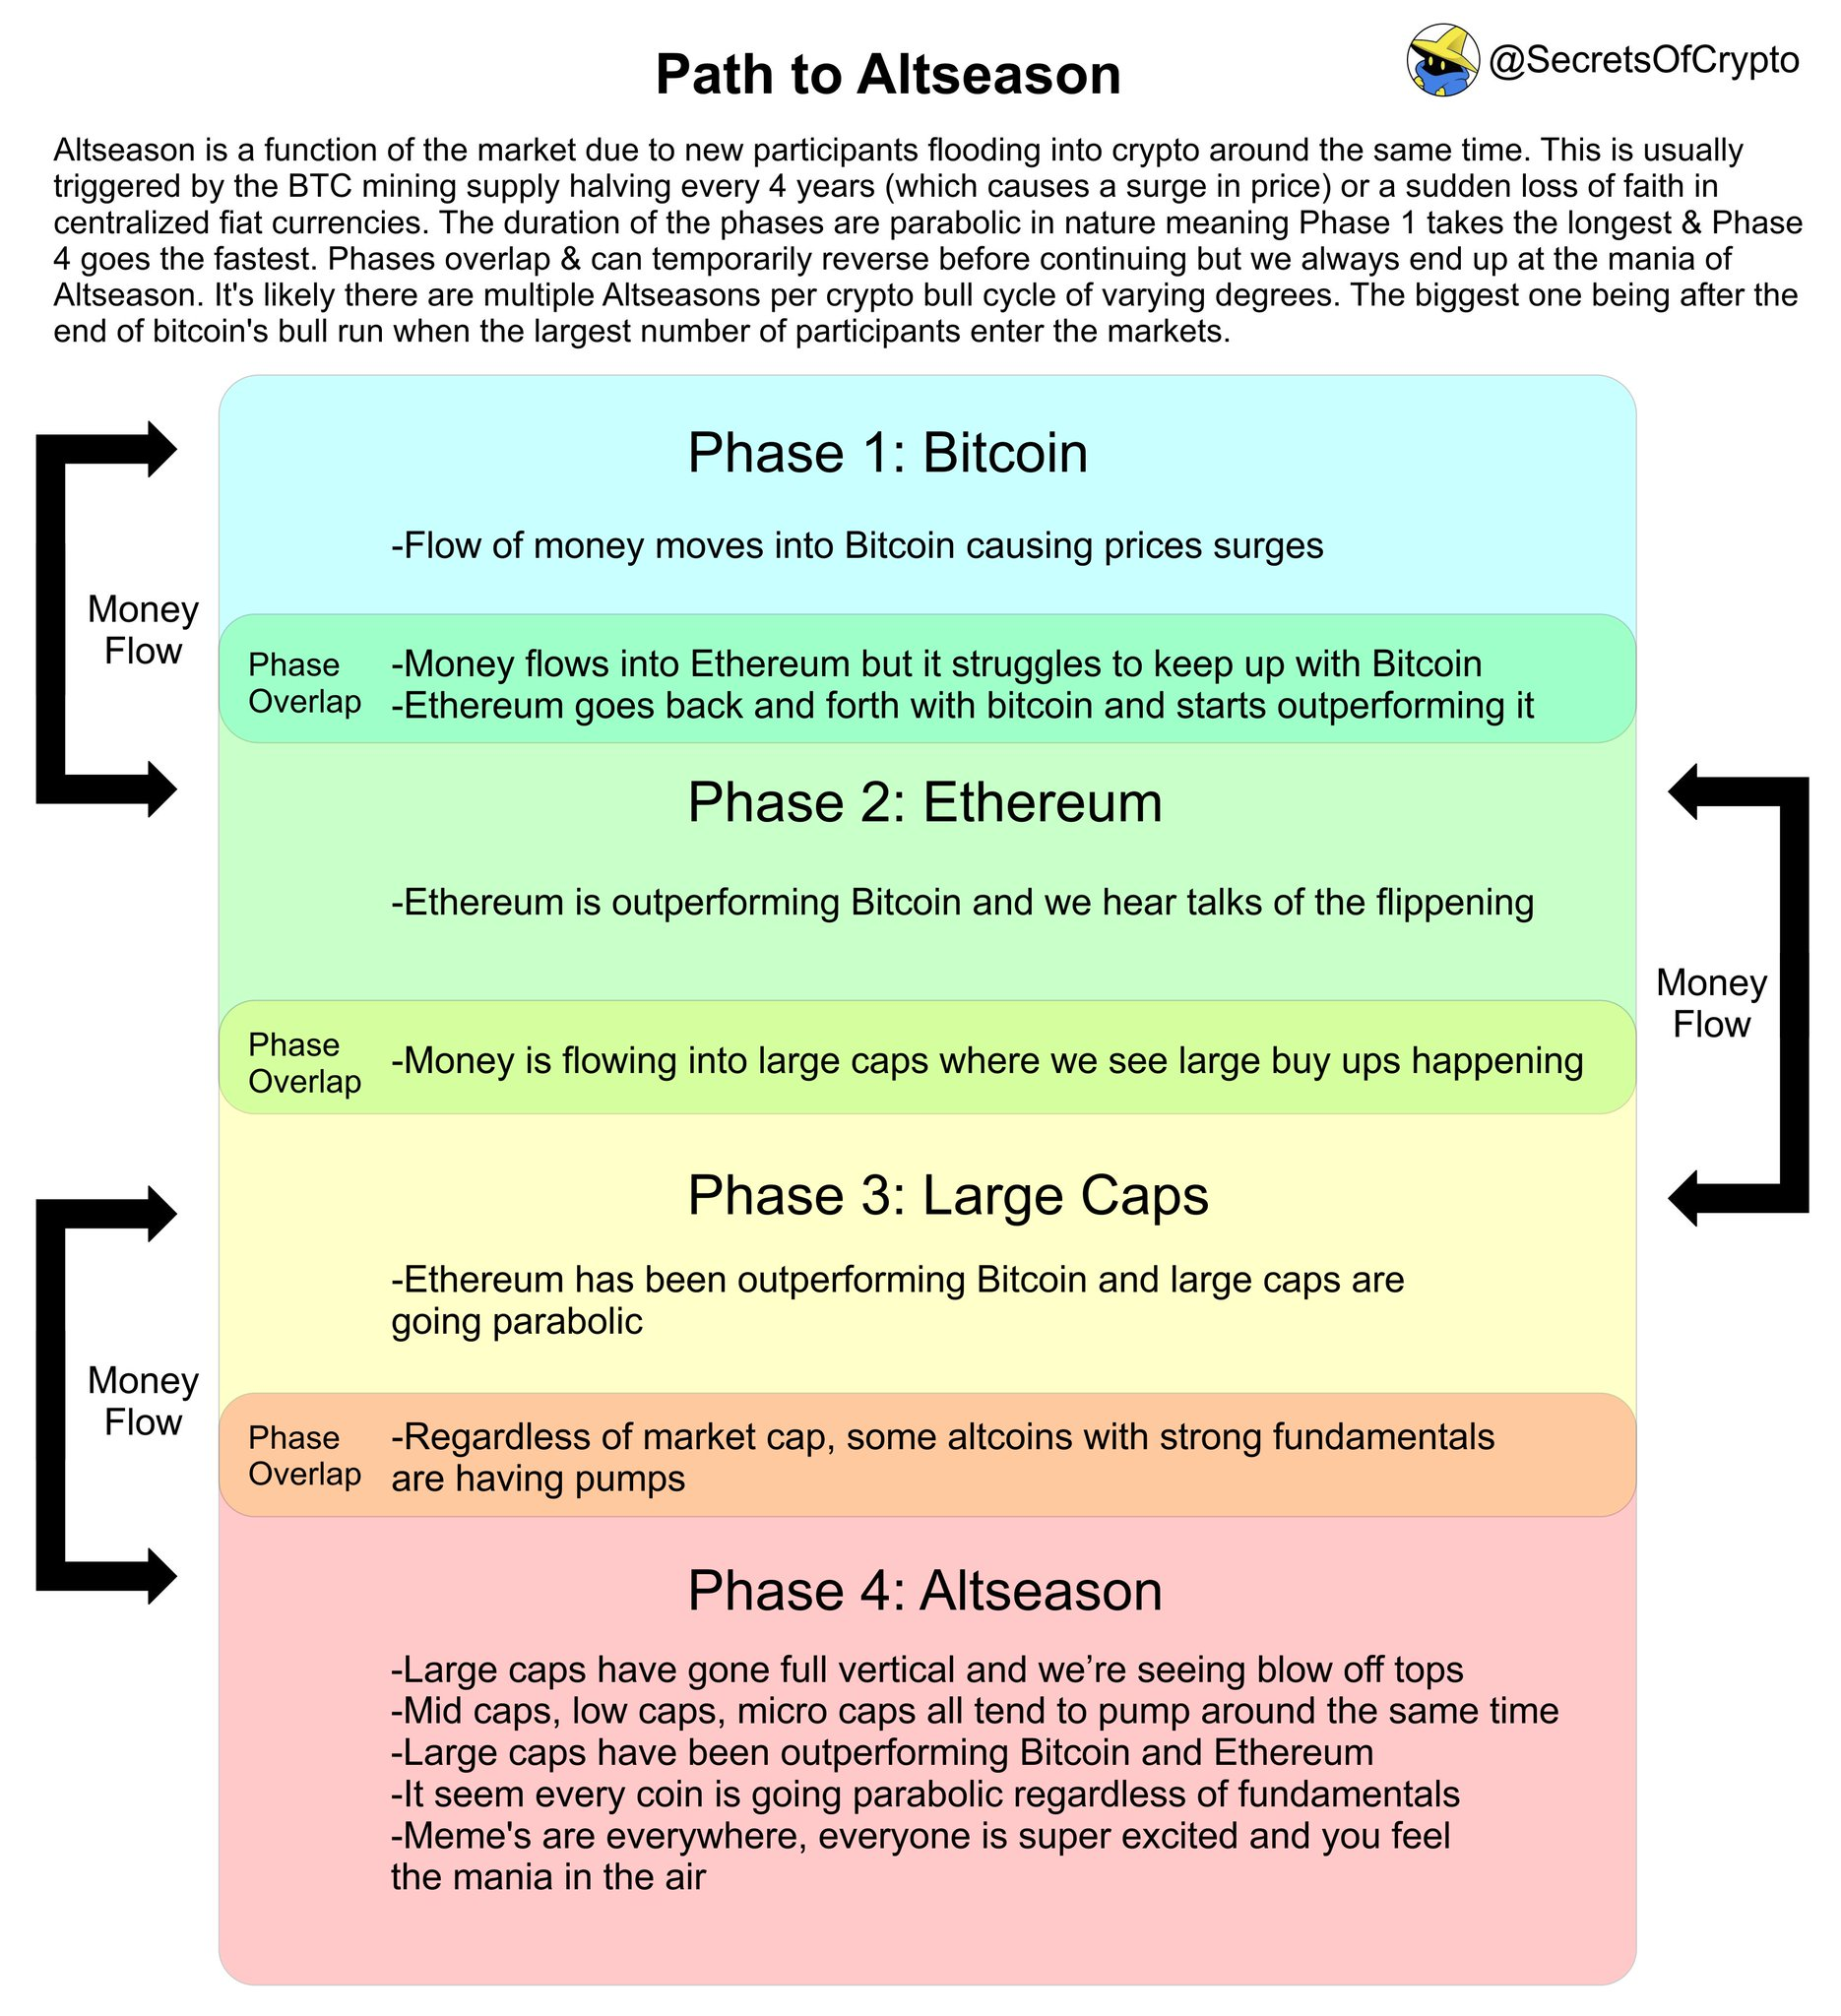
\includegraphics[width=0.5\linewidth]{path-to-altseason}

Bitcoin price action can cut this pattern short. Towards the end, a reliable signal for the top is when garbage coins pump across the board. 

\subsection{Dumb money vs smart money}
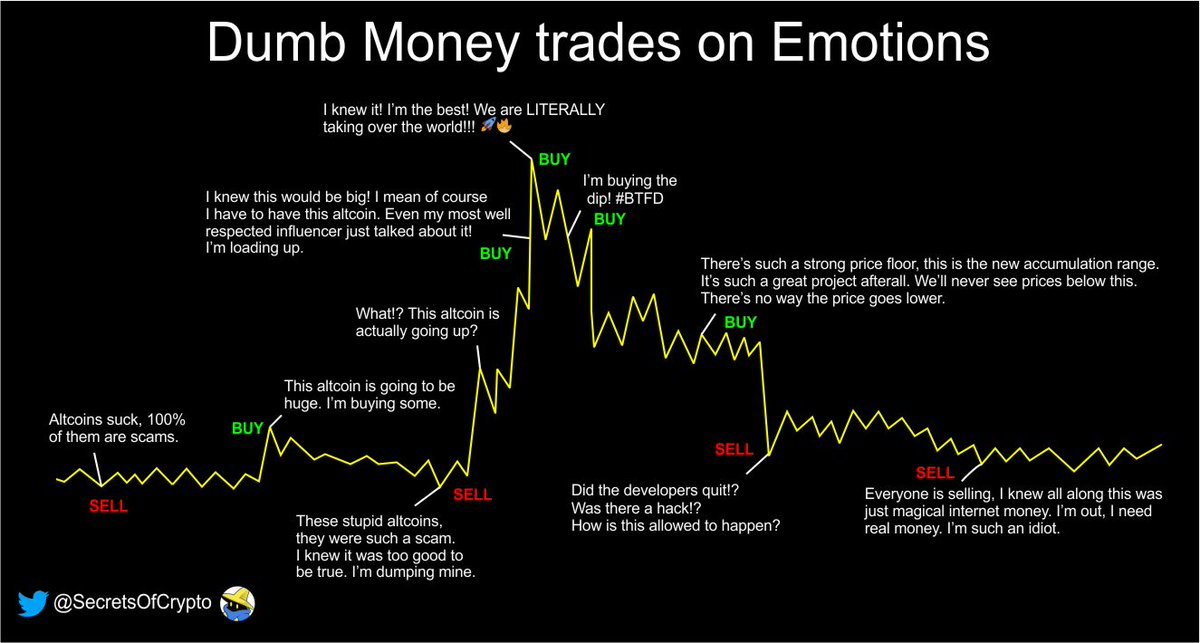
\includegraphics[width=0.5\linewidth]{dumb-money}
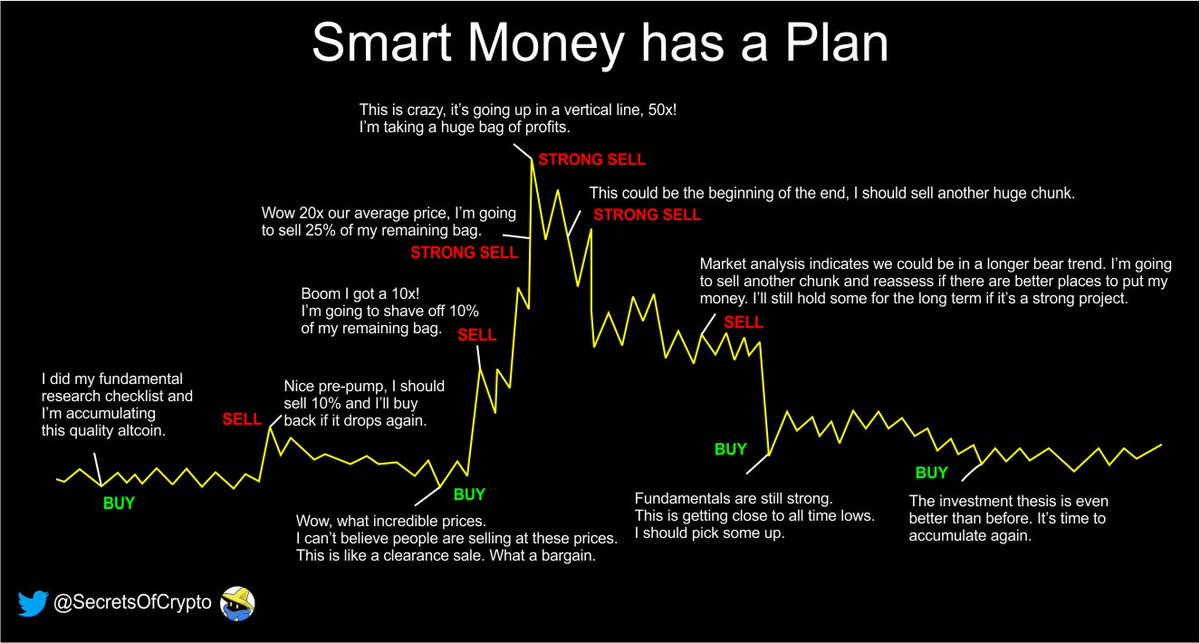
\includegraphics[width=0.5\linewidth]{smart-money}

\subsection{Flow of crowd for 4-year crypto cycle}
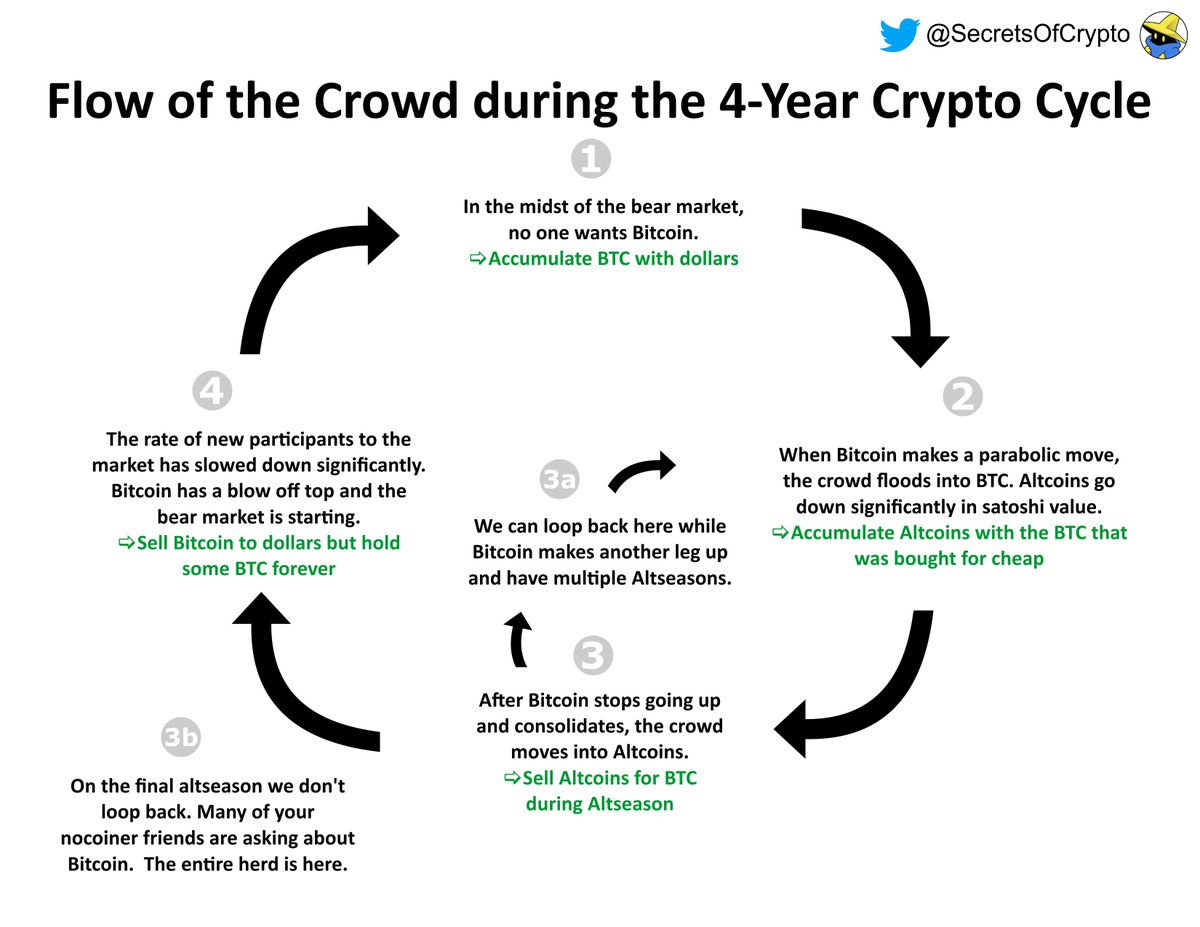
\includegraphics[width=0.5\linewidth]{crypto-cycle}
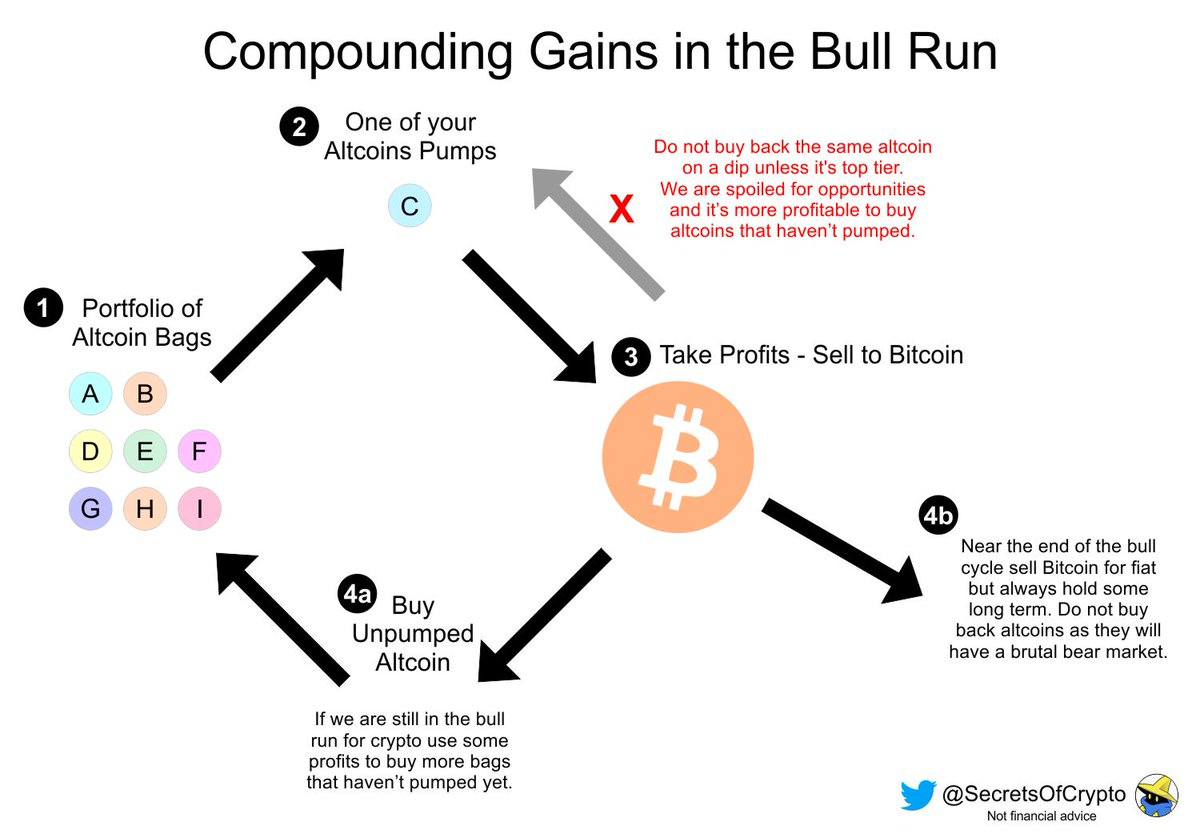
\includegraphics[width=0.5\linewidth]{bull-run-wealth}

\subsection{Altcoin Research Checklist}
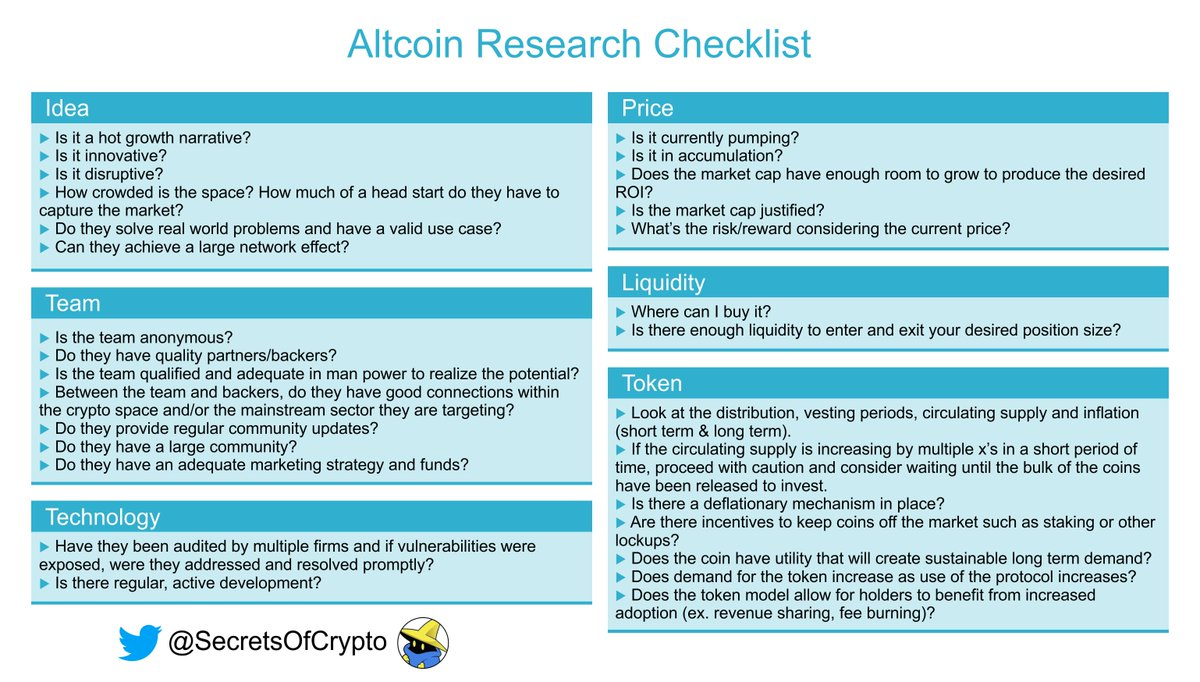
\includegraphics[width=0.6\linewidth]{altcoin-checklist}
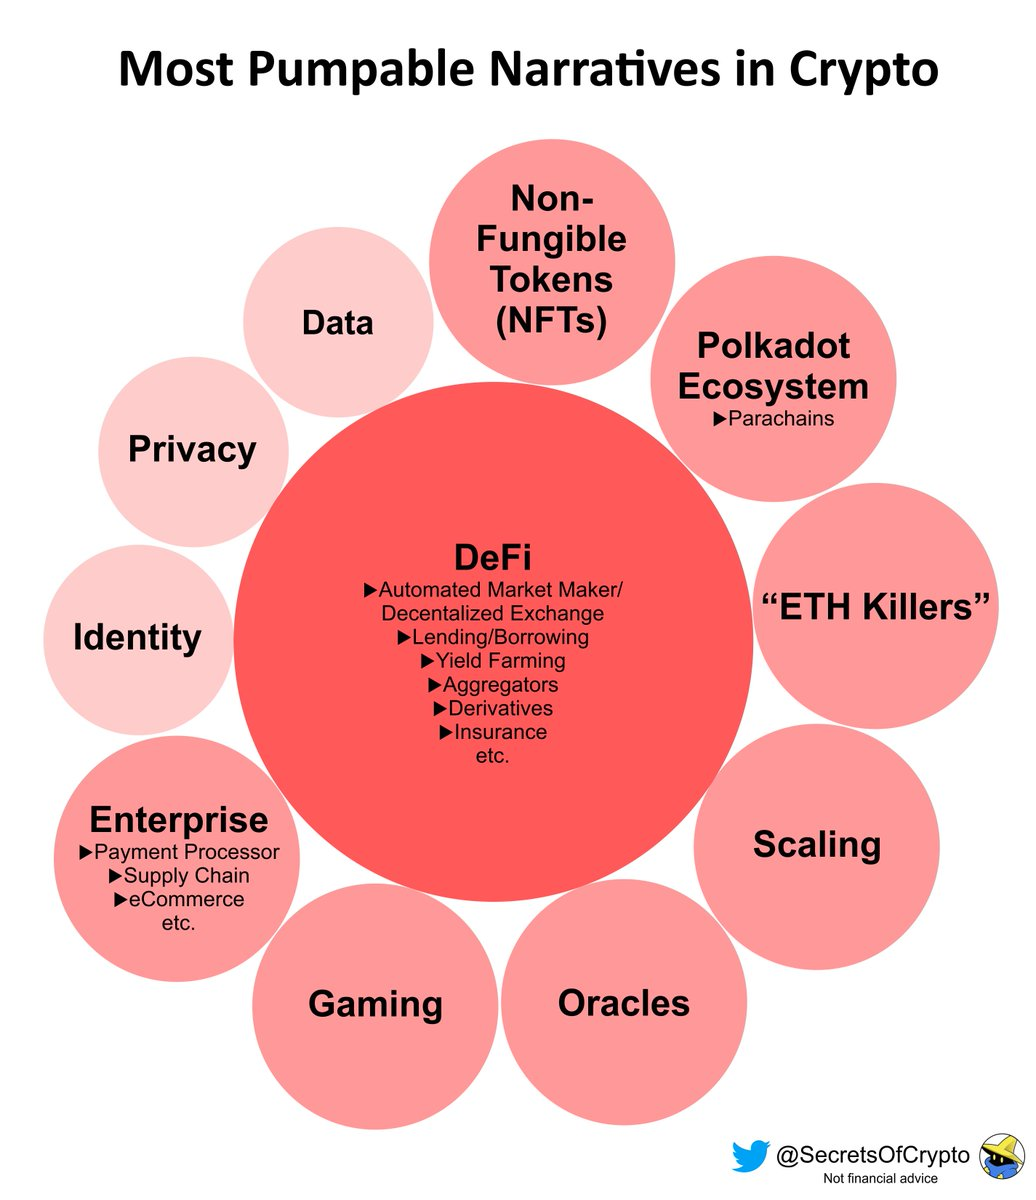
\includegraphics[width=0.4\linewidth]{pumpable-narratives}


\section{Copy-trading: We Like the Coins}
https://messari.io/article/messari-employee-holdings-policy-and-disclosures

Approx popularity: BTC, ETH, SOL, LUNA, HNT, RUNE, ATOM...Recommend rereading (page 19/165) their reasonings. May be very informative once I understand more. 





\end{document}
